% Deck de defensa — TFM Máster de Formación Permanente en Deep Learning (UPM)
% Compilar: tectonic -X compile defensa.tex
% Objetivo: 10-12 minutos. El guion oral vive en reports/defensa.md.
\documentclass[aspectratio=169,11pt]{beamer}

\usetheme{default}
\usecolortheme{default}
\setbeamertemplate{navigation symbols}{}
\setbeamertemplate{caption}{\insertcaption}

\usepackage[spanish,es-noshorthands]{babel}
\usepackage{fontspec}
\usepackage{booktabs}
\usepackage{graphicx}
\usepackage{tikz}
\usetikzlibrary{positioning,arrows.meta,calc,fit,backgrounds}

\graphicspath{{../memoria/figures/}}

% Paleta sobria, coherente con la memoria
\definecolor{tinta}{HTML}{1A1A1A}
\definecolor{azul}{HTML}{2B6CB0}
\definecolor{tierra}{HTML}{B45309}
\definecolor{verde}{HTML}{2F855A}
\definecolor{gris}{HTML}{6B7280}
\definecolor{fondo}{HTML}{FBFAF7}

\setbeamercolor{background canvas}{bg=fondo}
\setbeamercolor{structure}{fg=azul}
\setbeamercolor{frametitle}{fg=tinta}
\setbeamercolor{normal text}{fg=tinta}
\setbeamerfont{frametitle}{size=\large,series=\bfseries}
\setbeamertemplate{frametitle}{\vspace{0.7em}\insertframetitle\par
  \vspace{-0.35em}{\color{azul}\rule{0.12\textwidth}{1.2pt}}}

% Pie: número de diapositiva discreto
\setbeamertemplate{footline}{\hfill{\color{gris}\scriptsize\insertframenumber}\hspace{1.2em}\vspace{0.6em}}

% Frase clave al pie de una diapositiva
\newcommand{\clave}[1]{\vfill\noindent{\color{azul}\small\textbf{#1}}\par\vspace{0.2em}}
% Cifra grande
\newcommand{\cifra}[2]{{\color{#1}\Large\textbf{#2}}}

\title{Aprendizaje profundo aplicado a la microestructura de mercados de predicción}
\subtitle{Predicción de corto plazo en mercados de Bitcoin de Polymarket}
\author{Marc Maldonado Lorca}
\date{Septiembre de 2026}

\begin{document}

% ─────────────────────────────────────────────── 1. Portada
\begin{frame}[plain]
  \vspace{0.6em}
  \begin{center}
    
\includegraphics[height=1.5cm]{EscudoUPM.png}\hspace{2em}%
    
\includegraphics[height=1.5cm]{EscudoETSIAAB.png}
  \end{center}
  \vfill
  \begin{center}
    {\large\bfseries Aprendizaje profundo aplicado a la microestructura\\de mercados de predicción\par}
    \vspace{0.4em}
    {\color{gris}Predicción de corto plazo en mercados de Bitcoin de Polymarket}
    \vspace{1.4em}

    Marc Maldonado Lorca\\[0.3em]
    {\small\color{gris}Directora: Dra.\ María Inmaculada Santamaría Valenzuela}\\[0.2em]
    {\small\color{gris}Máster de Formación Permanente en Deep Learning · UPM}
  \end{center}
  \vfill
  \begin{center}
    {\color{azul}\small\textbf{No defiendo rentabilidad; defiendo una metodología de evaluación.}}
  \end{center}
  \vspace{0.8em}
\end{frame}

% ─────────────────────────────────────────────── 2. Problema
\begin{frame}{Qué se predice, exactamente}
  \begin{columns}[T]
    \begin{column}{0.52\textwidth}
      Un contrato binario de Polymarket \textbf{no es el precio de Bitcoin}. Es una
      probabilidad negociada: cuánto paga el mercado por un resultado futuro.

      \vspace{0.8em}
      En los mercados de Bitcoin está acoplado a referencias externas, y ese acoplamiento
      es lo que se estudia.

      \vspace{0.8em}
      {\color{tierra}\textbf{No predigo el evento final.}} Predigo movimientos locales del
      contrato, a escala de segundos.
    \end{column}
    \begin{column}{0.44\textwidth}
      \centering
      \begin{tikzpicture}[font=\scriptsize,
        n/.style={draw,rounded corners=2pt,minimum width=2.1cm,minimum height=0.62cm,align=center},
        f/.style={-{Stealth[length=2mm]},gris}]
        \node[n,fill=azul!8] (c) {contrato binario\\$p \in [0,1]$};
        \node[n,above left=0.75cm and -0.5cm of c] (s) {BTC \emph{spot}};
        \node[n,above right=0.75cm and -0.5cm of c] (p) {perpetuos};
        \node[n,below=0.75cm of c] (o) {oráculo};
        \draw[f] (s) -- (c); \draw[f] (p) -- (c); \draw[f] (o) -- (c);
        \node[below=0.15cm of o,text width=3.6cm,align=center,color=gris]
          {malla común de 2\,s};
      \end{tikzpicture}
    \end{column}
  \end{columns}
  \clave{Un contrato binario no es Bitcoin: hay que definir con precisión qué se predice.}
\end{frame}

% ─────────────────────────────────────────────── 3. Datos
\begin{frame}{El sistema de captura: la parte que decide qué se puede afirmar}
  \begin{columns}[T]
    \begin{column}{0.5\textwidth}
      Captura propia y continua que alinea cuatro fuentes en una malla de dos segundos,
      con control de calidad por sesión.

      \vspace{0.6em}
      \begin{itemize}\setlength\itemsep{0.25em}
        \item \cifra{azul}{2,5\,M} filas multifuente
        \item \cifra{azul}{50} días de ventana prospectiva
        \item Latencia medida contra el mercado real: \textbf{429,7\,ms} (p95), con una
              orden efectivamente casada
      \end{itemize}

      \vspace{0.6em}
      {\small La unidad no es un mercado: es una observación temporal con información
      causal hasta ese instante.}
    \end{column}
    \begin{column}{0.46\textwidth}
      \centering
      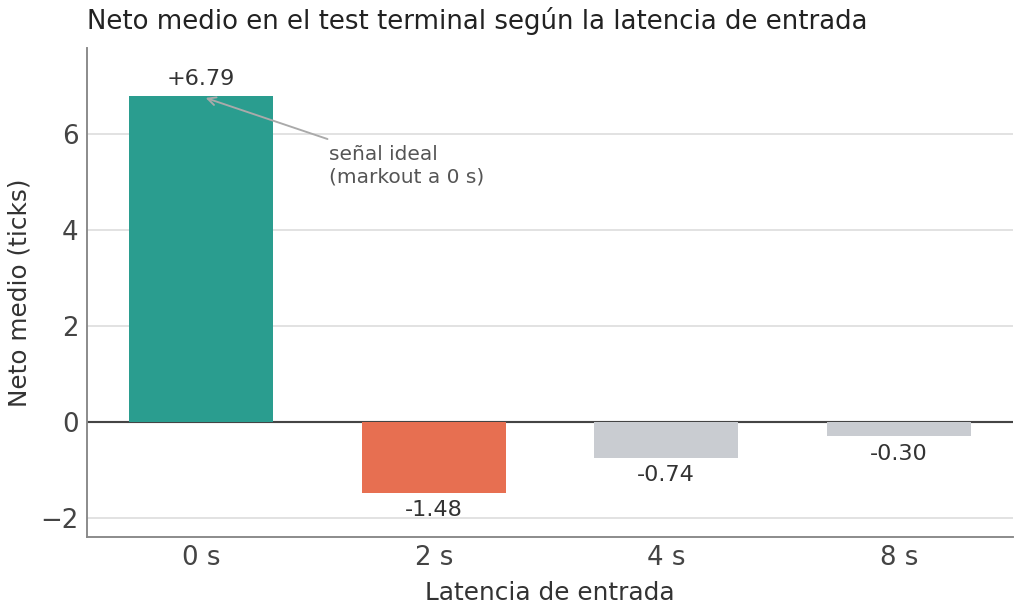
\includegraphics[width=\textwidth]{fig_latencia.png}
    \end{column}
  \end{columns}
  \clave{La parte de datos no es decorativa: define qué se puede afirmar después.}
\end{frame}

% ─────────────────────────────────────────────── 4. Protocolo
\begin{frame}{El protocolo está diseñado contra el autoengaño}
  \begin{columns}[T]
    \begin{column}{0.55\textwidth}
      \begin{itemize}\setlength\itemsep{0.45em}
        \item Particiones \textbf{estrictamente temporales}; características causales.
        \item El candidato se \textbf{congela} antes de ver el bloque de test.
        \item Todo se reporta en \textbf{ticks netos}: costes y latencia dentro.
        \item El compromiso se \textbf{sella en la cadena de Bitcoin} antes de mirar los
              datos (OpenTimestamps).
      \end{itemize}
      \vspace{0.5em}
      {\small\color{gris}Verificable por terceros: la atestación no se puede
      retro-fechar.}
    \end{column}
    \begin{column}{0.42\textwidth}
      \centering\scriptsize
      \begin{tikzpicture}[font=\tiny, x=0.82cm, y=0.55cm]
        \draw[gris,-{Stealth[length=2mm]}] (0,0) -- (7.2,0);
        \foreach \x/\t in {0.3/{11 may}, 2.5/{6 jun}, 4.3/{10 jul}, 6.4/{23 ago}}
          \draw[gris] (\x,-0.12) -- (\x,0.12) node[below=0.22cm,color=tinta] {\t};
        \draw[azul,line width=2pt] (0.3,0.55) -- (2.3,0.55)
          node[midway,above,color=azul] {entrenamiento};
        \draw[tierra,line width=2pt] (2.5,0.55) -- (3.3,0.55)
          node[midway,above,color=tierra] {test};
        \draw[verde,line width=2pt] (4.3,0.55) -- (6.4,0.55)
          node[midway,above,color=verde] {prospectivo};
        \node[gris,align=center] at (3.6,-1.15) {sellos previos a cada ventana};
      \end{tikzpicture}
    \end{column}
  \end{columns}
  \clave{La métrica que decide es económica, no la \emph{accuracy}.}
\end{frame}

% ─────────────────────────────────────────────── 5. El hallazgo central
\begin{frame}{Primer hallazgo: acertar no es ganar}
  \begin{columns}[c]
    \begin{column}{0.46\textwidth}
      \centering
      \vspace{0.4em}
      {\color{verde}\Huge\textbf{$\approx$90\,\%}}\\[0.2em]
      {\small acierto direccional}\\[1.6em]
      {\color{tierra}\Huge\textbf{negativo}}\\[0.2em]
      {\small resultado económico con 2\,s de latencia}
    \end{column}
    \begin{column}{0.5\textwidth}
      El primer \emph{baseline} tabular parecía excelente mirando solo la clasificación.
      Introduciendo el retardo de entrada, el resultado se vuelve negativo.

      \vspace{0.8em}
      Eso cambia el eje del trabajo: no basta con acertar la dirección, hay que entrar a un
      precio que todavía permita capturar valor.

      \vspace{0.8em}
      {\small\color{gris}Precisión sobre el alcance: los 2\,s son la resolución del
      instrumento, no la latencia medida. Entre 0 y 2\,s no hay observaciones.}
    \end{column}
  \end{columns}
  \clave{El modelo puede tener razón demasiado tarde.}
\end{frame}

% ─────────────────────────────────────────────── 6. Escalera de modelos
\begin{frame}{La escalera de modelos: el aprendizaje profundo sí se evaluó}
  \begin{columns}[T]
    \begin{column}{0.52\textwidth}
      \small
      \begin{itemize}\setlength\itemsep{0.3em}
        \item Tabulares regularizados · sensibles a latencia
        \item GRU, \emph{BookEncoder} convolucional (DeepLOB), fusión, TCN, auto-atención
        \item Fundacionales: \textbf{MOMENT} (series) y \textbf{TabPFN} (tabular)
      \end{itemize}
      \vspace{0.8em}
      MOMENT mejora de forma monótona al adaptarlo y aun así no bate a la deriva ingenua
      ni a un ARIMA; su curva de escalado es \textbf{plana}.

      \vspace{0.5em}
      TabPFN gana la \textbf{ordenación} \emph{zero-shot} con un tercio de los datos
      (Spearman 0,119 frente a 0,092), pero no mejora la decisión ni la vuelve rentable.
    \end{column}
    \begin{column}{0.44\textwidth}
      \centering
      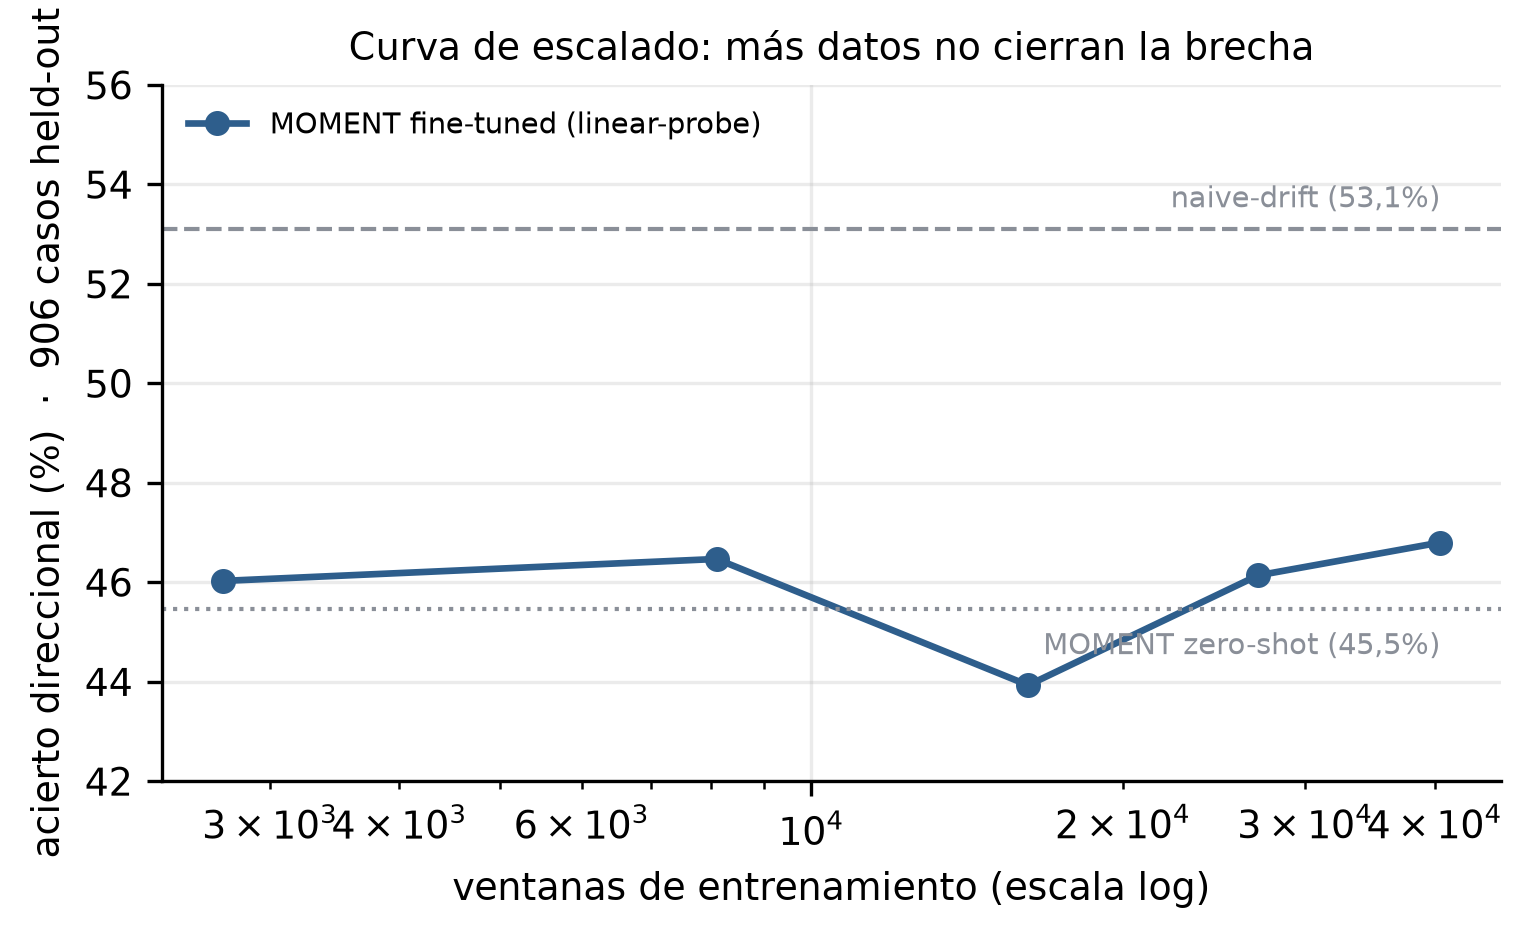
\includegraphics[width=\textwidth]{fig_moment_scaling.png}
    \end{column}
  \end{columns}
  \clave{La complejidad no se da por buena: debe ganarse su sitio.}
\end{frame}

% ─────────────────────────────────────────────── 7. Candidato final
\begin{frame}{El candidato congelado}
  \begin{columns}[T]
    \begin{column}{0.5\textwidth}
      Especialista para la ventana \emph{prestart}, entre $-60$ y $-45$\,s de la apertura.
      36 características causales, sin variables de reloj.

      \vspace{0.8em}
      Dos cabezas y una regla que exige ambas condiciones:
      \begin{itemize}\setlength\itemsep{0.2em}
        \item valor esperado $> 0{,}75$
        \item probabilidad de relleno sano $\ge 0{,}50$
      \end{itemize}

      \vspace{0.8em}
      {\small\color{gris}No intenta operar todo: intenta seleccionar contextos
      ejecutables.}
    \end{column}
    \begin{column}{0.46\textwidth}
      \centering
      \begin{tikzpicture}[font=\scriptsize,
        b/.style={draw,rounded corners=2pt,minimum width=2.4cm,minimum height=0.7cm,align=center},
        f/.style={-{Stealth[length=2mm]},gris}]
        \node[b,fill=azul!8] (x) {36 características\\causales};
        \node[b,below left=0.9cm and -0.9cm of x] (ev) {cabeza EV};
        \node[b,below right=0.9cm and -0.9cm of x] (he) {cabeza salud};
        \node[b,below=2.5cm of x,fill=verde!10] (r) {operar sólo si\\ambas se cumplen};
        \draw[f] (x) -- (ev); \draw[f] (x) -- (he);
        \draw[f] (ev) -- (r); \draw[f] (he) -- (r);
      \end{tikzpicture}
    \end{column}
  \end{columns}
  \clave{Selecciona contextos ejecutables, no oportunidades en abstracto.}
\end{frame}

% ─────────────────────────────────────────────── 8. Fe de erratas
\begin{frame}{La fe de erratas que refuerza la tesis}
  \begin{columns}[T]
    \begin{column}{0.48\textwidth}
      \centering
      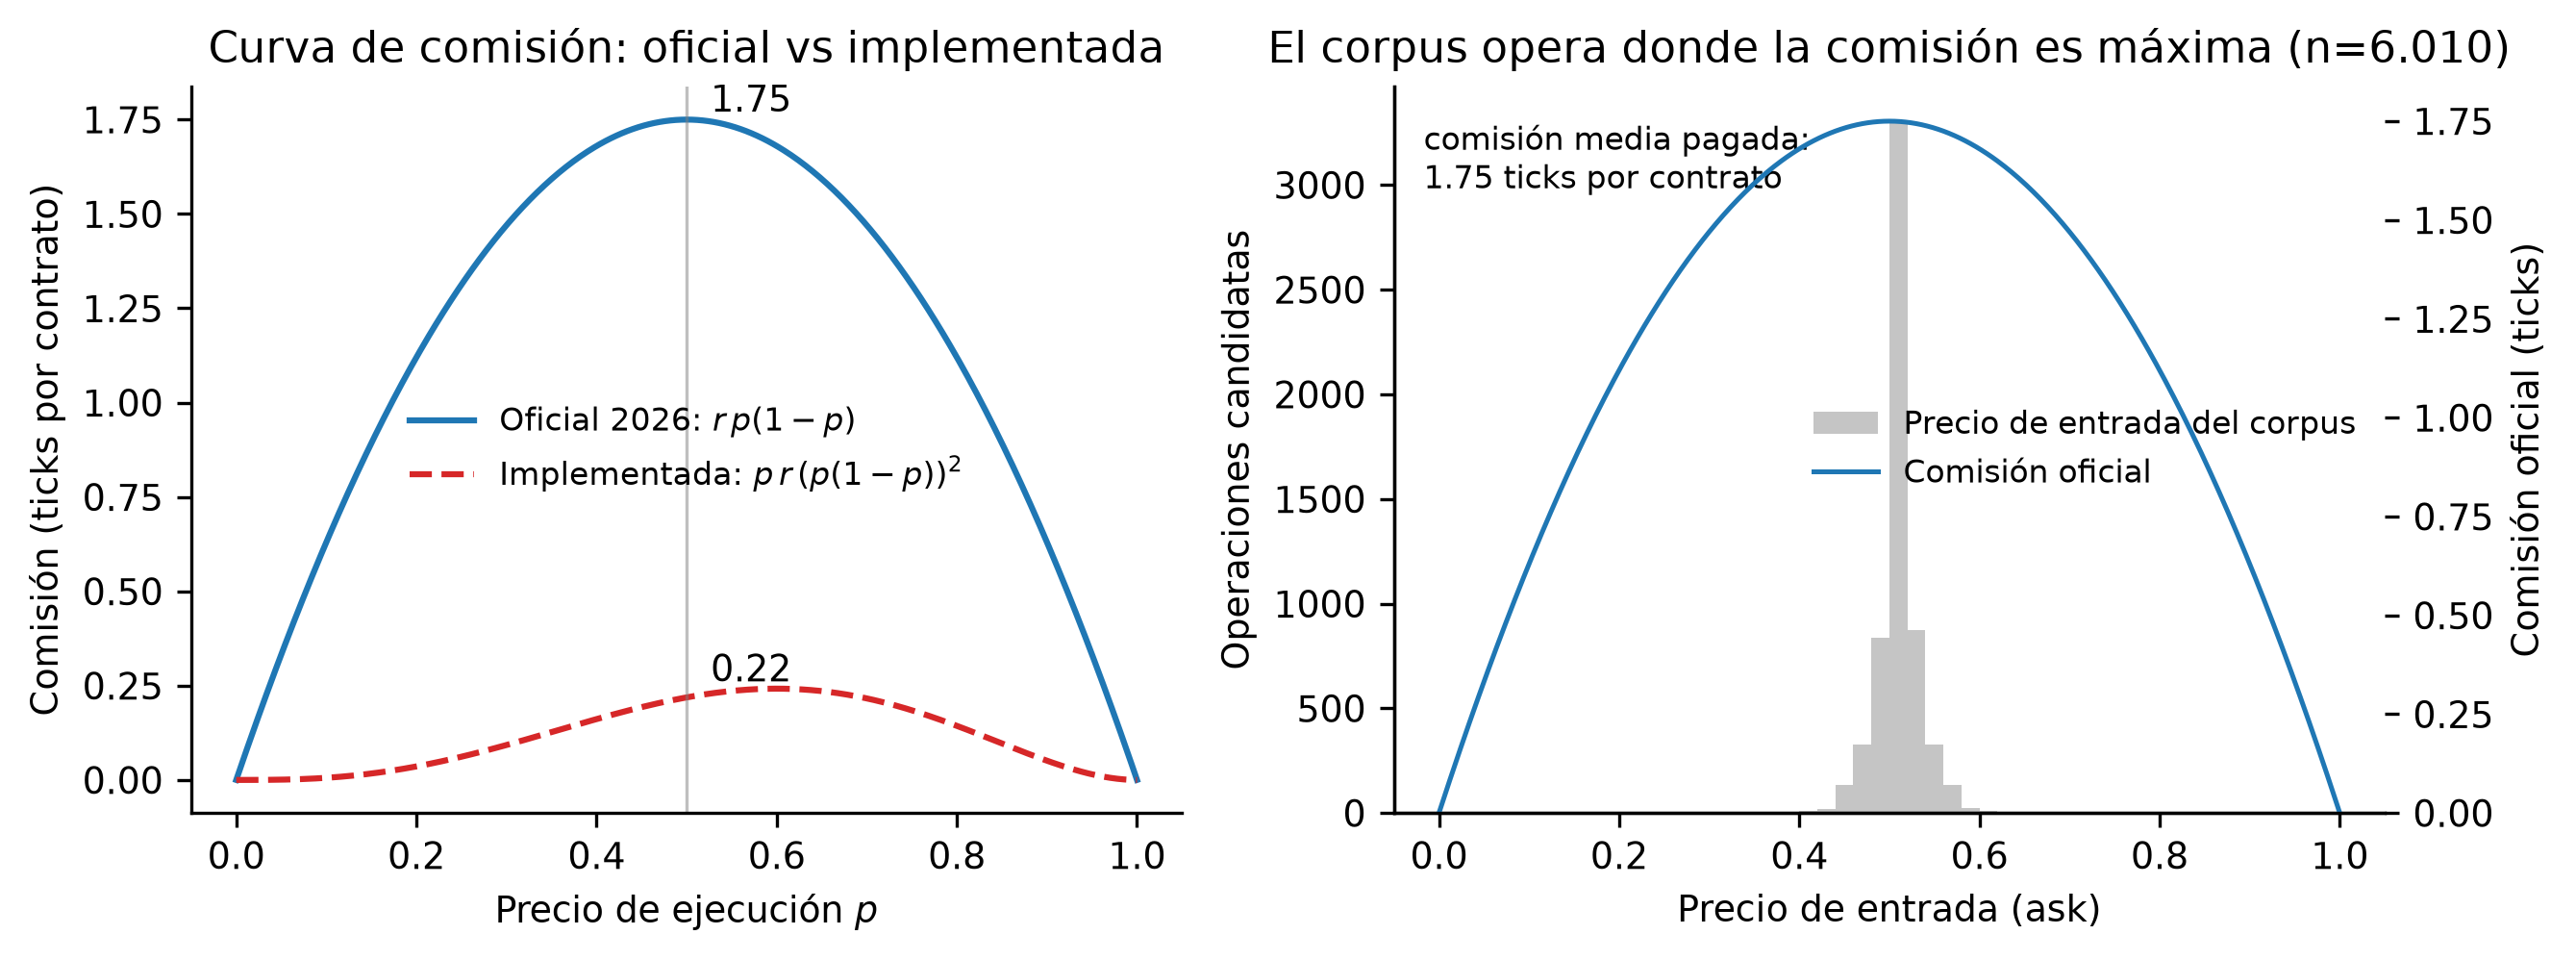
\includegraphics[width=\textwidth]{fig_fees_errata.png}
    \end{column}
    \begin{column}{0.48\textwidth}
      En la fase final detecté que mi modelo subestimaba la comisión \emph{taker} en un
      \textbf{factor ocho}, justo en la zona de precios donde opera el trabajo.

      \vspace{0.6em}
      Lo declaré como fe de erratas \textbf{sellada}, y re-evalué la política congelada sin
      reentrenar nada:

      \vspace{0.4em}
      \centering\scriptsize
      \begin{tabular}{lrr}
        \toprule
         & entrada & ida y vuelta \\
        \midrule
        Todas ($n{=}754$) & $-1{,}059$ & $-3{,}304$ \\
        Baja vol. ($n{=}318$) & $-0{,}342$ & $-2{,}604$ \\
        \bottomrule
      \end{tabular}

      \vspace{0.6em}
      \raggedright La comisión media de entrada, $1{,}75$ ticks, \textbf{supera por sí sola}
      el resultado bruto de la señal.
    \end{column}
  \end{columns}
  \clave{El error, declarado y sellado, confirma la tesis.}
\end{frame}

% ─────────────────────────────────────────────── 9. Giro maker
\begin{frame}{El valor no desaparece: se desplaza al otro lado del libro}
  \begin{columns}[T]
    \begin{column}{0.5\textwidth}
      La misma estructura de comisiones que mata al \emph{taker} \textbf{retribuye} a quien
      provee liquidez: exento de comisión y con una parte del fondo de \emph{rebates}.

      \vspace{0.7em}
      Construí un simulador de colas y \emph{fills} para evaluarlo sin operar. Dos
      hallazgos de diseño:

      \begin{itemize}\setlength\itemsep{0.25em}
        \item la selección adversa de corto plazo es \textbf{favorable} al maker;
        \item el riesgo vive en el \textbf{inventario terminal}, no en el \emph{spread}.
      \end{itemize}
    \end{column}
    \begin{column}{0.46\textwidth}
      \centering
      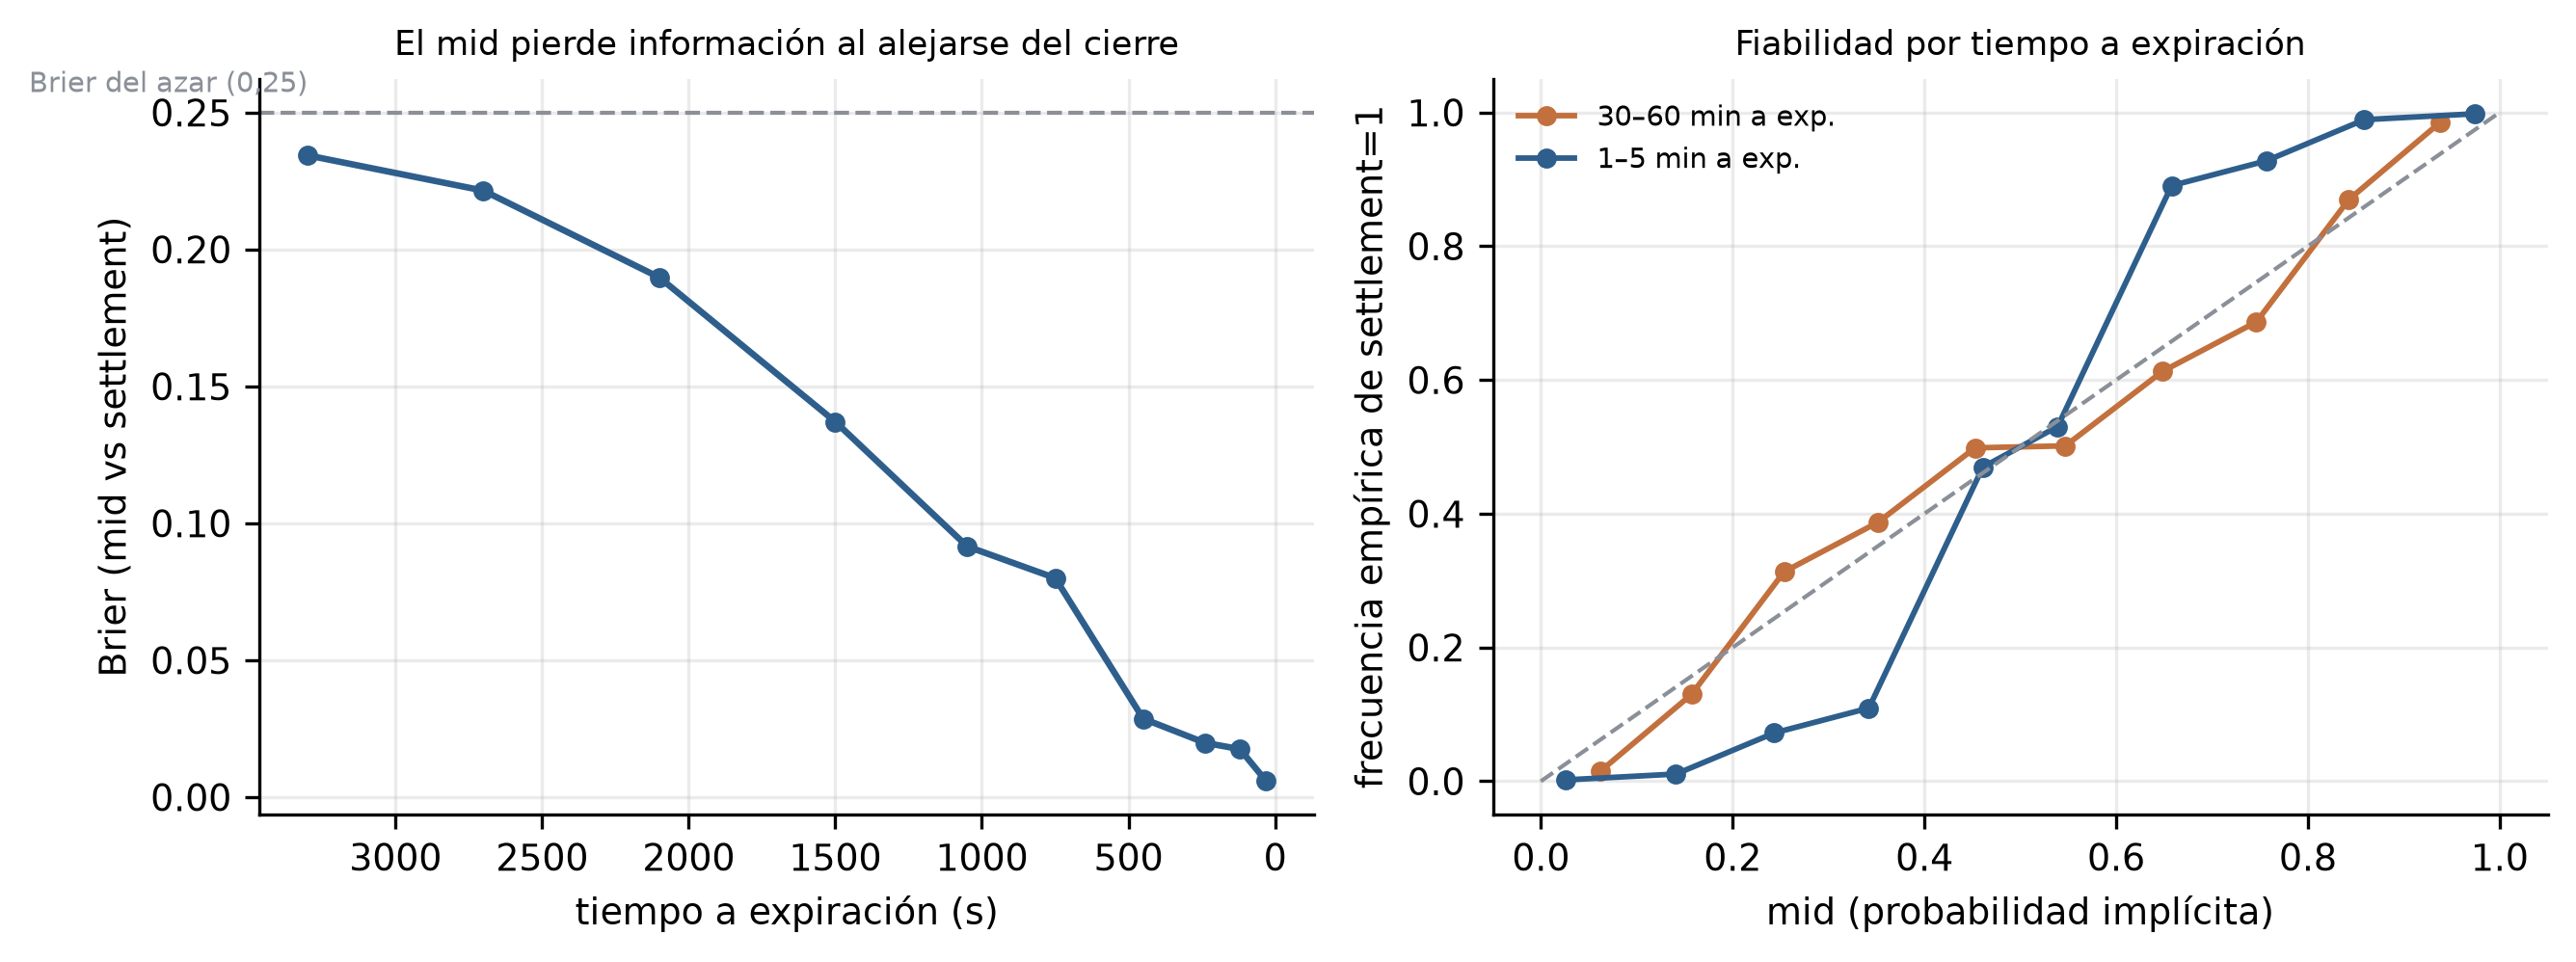
\includegraphics[width=\textwidth]{fig_n1_calibracion_terminal.png}\\[0.3em]
      {\scriptsize\color{gris}En la apertura el precio es casi una moneda al aire; sólo en
      el tramo terminal se vuelve resolutivo.}
    \end{column}
  \end{columns}
  \clave{El vehículo viable es cobrar el \emph{spread}, no pagarlo.}
\end{frame}

% ─────────────────────────────────────────────── 10. Validación prospectiva maker
\begin{frame}{Validación prospectiva pre-registrada: NO-GO}
  \begin{columns}[T]
    \begin{column}{0.47\textwidth}
      \centering
      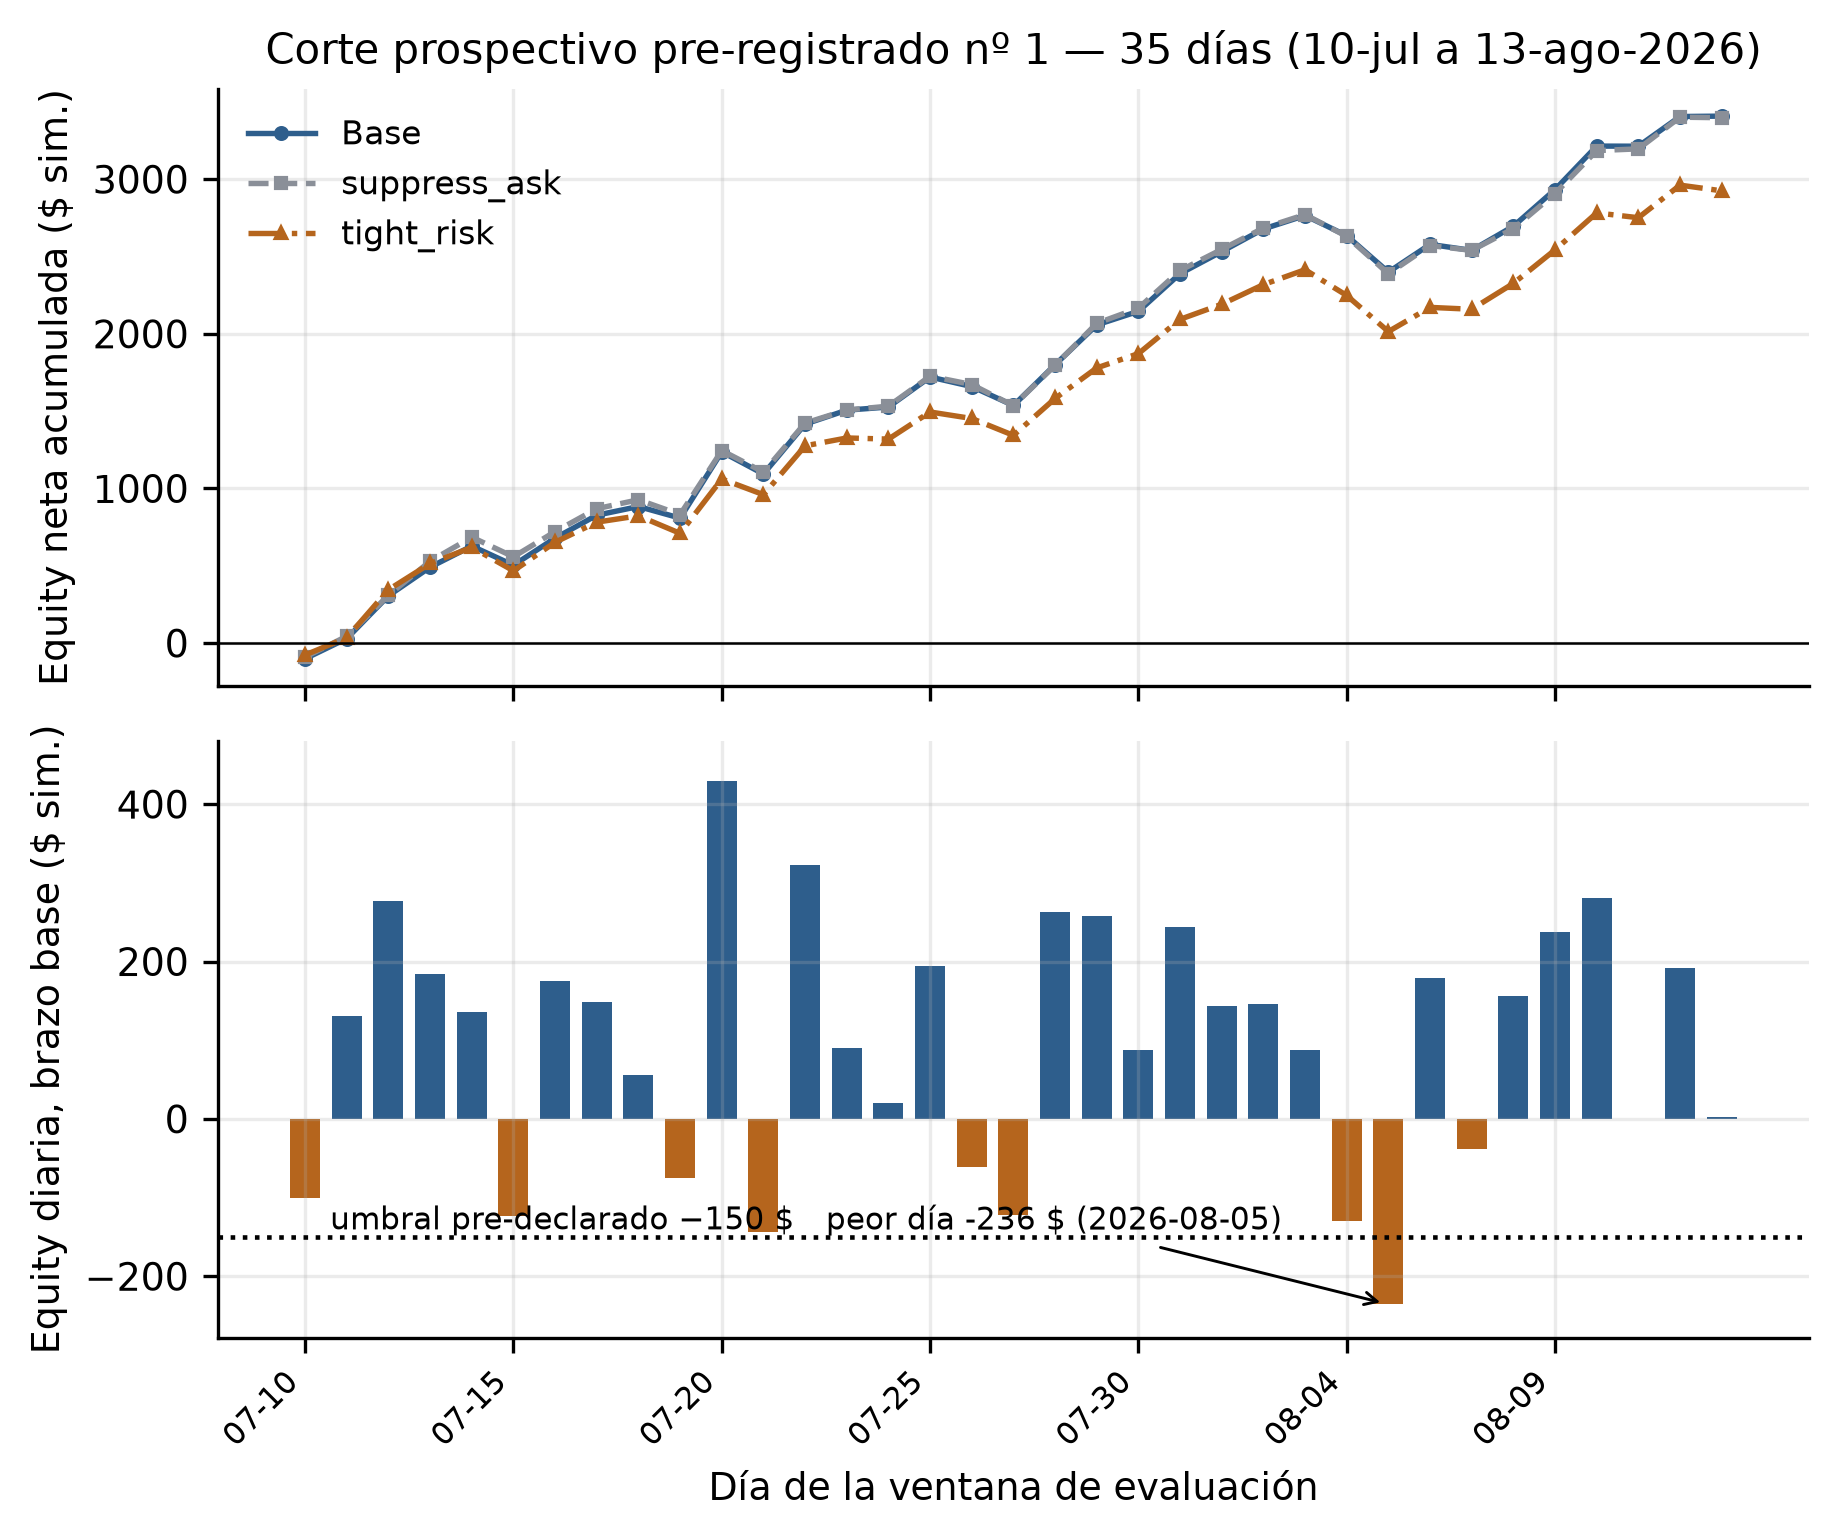
\includegraphics[width=\textwidth]{fig_corte_prospectivo.png}
    \end{column}
    \begin{column}{0.49\textwidth}
      Una sola corrida sobre 35 días posteriores al sello. La política \textbf{gana dinero}
      —$+3.408$\,\$ simulados— y aun así el veredicto es \textbf{NO-GO}: su peor día,
      $-235{,}66$\,\$, cruza el umbral declarado de $-150$.

      \vspace{0.6em}
      {\color{tierra}\textbf{Y aquí está lo incómodo:}} esa puerta se falla el
      \textbf{63--87\,\%} de las veces \emph{con independencia de la calidad de la
      política}. El sub-criterio que firmó el veredicto era el único sin potencia; el que
      sí la tenía se cumplía con holgura.

      \vspace{0.4em}
      {\small\color{gris}La ventana la cerró un fallo de hardware, no yo.}
    \end{column}
  \end{columns}
  \clave{Una regla pre-registrada sólo vale si se obedece cuando incomoda.}
\end{frame}

% ─────────────────────────────────────────────── 11. Corte del protocolo general
\begin{frame}{El cuarto camino, y el que por fin tiene potencia}
  \begin{columns}[T]
    \begin{column}{0.52\textwidth}
      \small
      \begin{tabular}{lrr}
        \toprule
        \textbf{Capa} & \textbf{Media} & \textbf{IC 95\,\%} \\
        \midrule
        Histórica @0,5 & $-0{,}004$ & $[-0{,}22;\ +0{,}21]$ \\
        Con comisión real & $-0{,}770$ & $[-0{,}99;\ -0{,}55]$ \\
        \emph{Taker} entrada & $-1{,}411$ & $[-1{,}63;\ -1{,}20]$ \\
        \emph{Taker} ida-vuelta & $-3{,}646$ & $[-3{,}87;\ -3{,}43]$ \\
        \bottomrule
      \end{tabular}

      \vspace{0.5em}
      {\scriptsize 50 días · 25.011 unidades · IC agrupado por mercado}
    \end{column}
    \begin{column}{0.44\textwidth}
      La cifra que este corte venía a contrastar —los $+0{,}349$ de junio—
      \textbf{nunca fue significativa}: su IC es $[-0{,}19;\ +0{,}89]$.

      \vspace{0.7em}
      Así que no hay deterioro que explicar. Con \textbf{33 veces más datos} la señal sigue
      sin distinguirse del azar, y la comisión vigente la vuelve decisivamente negativa.
    \end{column}
  \end{columns}
  \clave{Por fin potencia para afirmar la ausencia, no sólo para sugerirla.}
\end{frame}

% ─────────────────────────────────────────────── 12. Entrenar contra el dinero
\begin{frame}{¿Y si el problema era el objetivo, no la arquitectura?}
  \begin{columns}[T]
    \begin{column}{0.5\textwidth}
      Censo de las funciones de pérdida de todo el trabajo:

      \vspace{0.4em}
      {\small BCE ($\times$18) · L1 ($\times$16) · QLIKE ($\times$15) ·
      \textbf{económicas ($\times$0)}}

      \vspace{0.7em}
      Todos los modelos entrenaban contra una pérdida estadística y decidían después con un
      umbral. La última línea entrena la \textbf{decisión} directamente contra el dinero,
      con el contrafactual exacto de cada acción y la puerta de riesgo escrita como función
      de pérdida.

      \vspace{0.6em}
      {\small\color{gris}El \emph{sizing} continuo se descartó por medición: la caja no es
      monótona en el tamaño.}
    \end{column}
    \begin{column}{0.46\textwidth}
      \centering
      \vspace{1em}
      {\color{tierra}\Large\textbf{0 de 16}}\\[0.3em]
      {\small puntos de la frontera aprendida\\que batan a un parámetro escalar}

      \vspace{1.4em}
      Tras agotar los tres ejes —arquitectura, datos y objetivo— la conclusión ya no es que
      falte capacidad.
    \end{column}
  \end{columns}
  \clave{Para esta decisión, el mejor modelo resultó ser un número bien elegido.}
\end{frame}

% ─────────────────────────────────────────────── 13. Limitaciones
\begin{frame}{Los límites, declarados, son parte del resultado}
  \begin{columns}[T]
    \begin{column}{0.49\textwidth}
      \begin{itemize}\setlength\itemsep{0.35em}
        \item El simulador asume que los \emph{makers} incumbentes \textbf{no reaccionan} a
              mis órdenes. Ningún \emph{replay} puede medir esa respuesta.
        \item Dos tercios de las órdenes casadas dependen de un mecanismo declarado
              \textbf{optimista}.
        \item La malla de 2\,s no permite observar el intervalo donde vive la latencia
              realmente medida.
      \end{itemize}
    \end{column}
    \begin{column}{0.47\textwidth}
      \begin{itemize}\setlength\itemsep{0.35em}
        \item El suceso que hay que aprender a evitar —el día de pérdida severa— es tan raro
              que \textbf{las particiones pequeñas lo pierden}: una validación de una semana
              sale limpia el 43\,\% de las veces.
        \item Reproducibilidad parcial: el corpus completo no se publica por tamaño.
      \end{itemize}
      \vspace{0.5em}
      {\small\color{gris}Por eso no se reporta ROI, sino ticks netos y soporte.}
    \end{column}
  \end{columns}
  \clave{No convertir un diagnóstico retrospectivo en una promesa económica.}
\end{frame}

% ─────────────────────────────────────────────── 14. Aportaciones
\begin{frame}{Aportaciones}
  \begin{columns}[T]
    \begin{column}{0.48\textwidth}
      \begin{enumerate}\setlength\itemsep{0.4em}
        \item Sistema de captura multifuente con control de calidad por sesión, y el corpus
              alineado que produce.
        \item Protocolo de evaluación con costes y latencia medidos, \textbf{pre-registrado
              y sellado en la cadena de Bitcoin}.
      \end{enumerate}
    \end{column}
    \begin{column}{0.48\textwidth}
      \begin{enumerate}\setcounter{enumi}{2}\setlength\itemsep{0.4em}
        \item Evidencia por \textbf{cuatro caminos independientes} de la ruptura entre
              predicción y ejecución.
        \item Trazabilidad de los resultados negativos y de las correcciones, con la misma
              dignidad que los positivos.
      \end{enumerate}
    \end{column}
  \end{columns}
  \vspace{0.8em}
  {\small La aportación no es «este modelo gana», sino un marco reproducible para evaluar
  señales de microestructura en mercados de predicción.}
  \clave{La metodología es el entregable.}
\end{frame}

% ─────────────────────────────────────────────── 15. Cierre
\begin{frame}[plain]
  \vspace{2.2em}
  \begin{center}
    {\large Hay señal, pero es frágil.}\\[0.5em]
    {\large La ejecución importa más que la precisión.}\\[0.5em]
    {\large Cualquier afirmación económica necesita datos nuevos.}
  \end{center}
  \vfill
  \begin{center}
    {\color{azul}\Large\textbf{En microestructura, una predicción sólo cuenta\\si sobrevive al mercado.}}
  \end{center}
  \vfill
  \begin{center}
    {\small\color{gris}Queda sellada una confirmación prospectiva con mirada única,
    pendiente de ejecutarse sobre datos que nadie ha visto.}
  \end{center}
  \vspace{1.4em}
\end{frame}

\end{document}
